\documentclass[]{report}
\usepackage{ctex}
\usepackage{graphicx}
\usepackage{amssymb}
\usepackage{amsmath}

% Title Page
\title{操作系统作业PA1 实验报告}
\author{221900180 田永铭}


\begin{document}
\maketitle

\section{虚拟机创建和系统安装过程描述}

{\bf 1.下载qemu} 原本在ubuntu虚拟机内,通过指令下载并且编译,不过缺失太多依赖,安装失败。后选择在qemu官网下载exe直接运行,取得成功。

{\bf 2.下载镜像} 分别从微软官网下载windows-7镜像和Ubuntu官网下载ubuntu-22镜像。

\begin{figure}[h!]
	\centering
	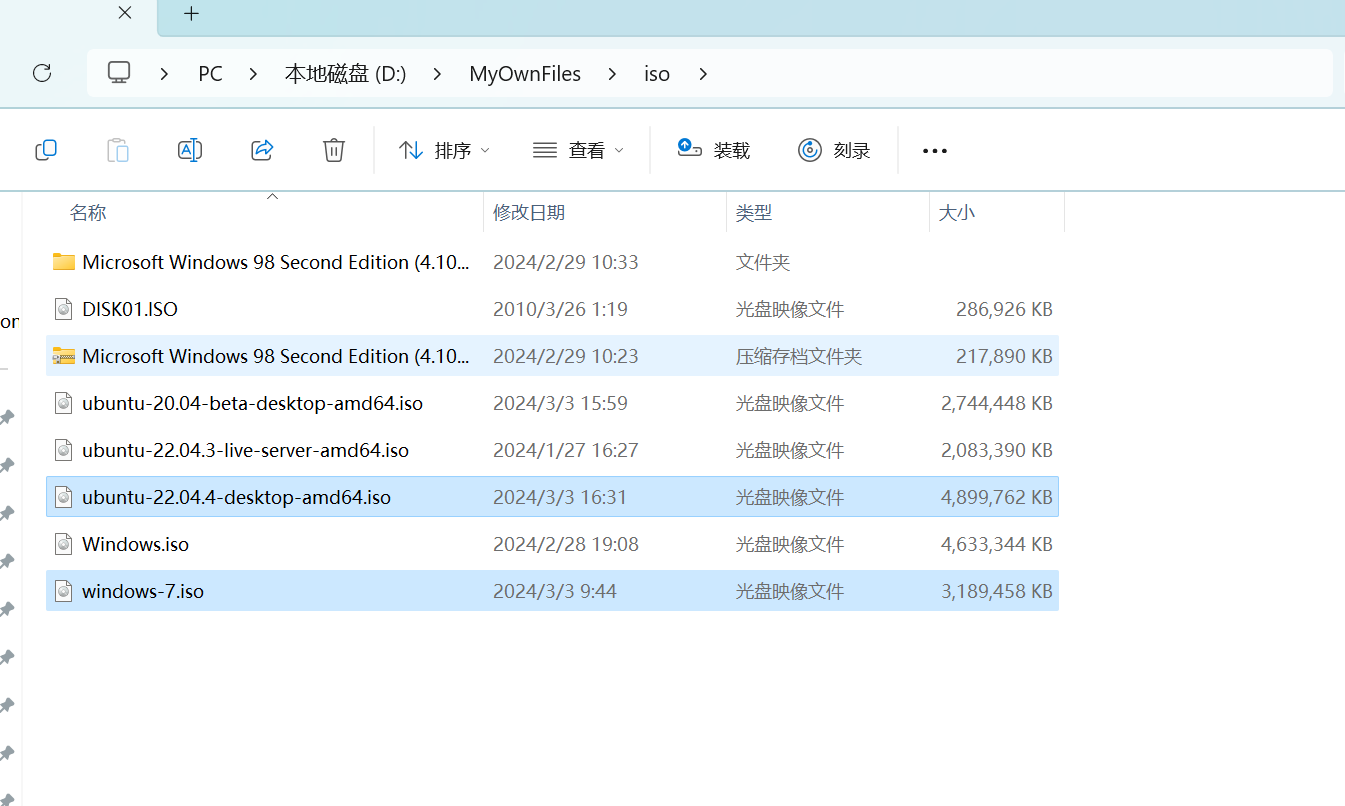
\includegraphics[width=0.7\linewidth]{C:/Users/86181/Desktop/pictures/0}
	\caption{下载的镜像如上图所示,选中的下面两个为实际采纳的}
	\label{fig:0}
\end{figure}

{\bf 3.先安装windows操作系统} 在qemu文件位置打开cmd,输入``qemu-img create os.img 35G"创建一个虚拟磁盘,再输入``qemu-system-x86\_64 -m 2048 -smp 2 os.img D:$\backslash$MyOwnFiles$\backslash$iso$\backslash$windows-7.iso"命令进行安装(后面跟的路径为本地iso文件地址)。安装时,进行磁盘分区,预留出一半空间给linux系统。下图为安装成功的windows-7图片展示。
\begin{figure}[h!]
	\centering
	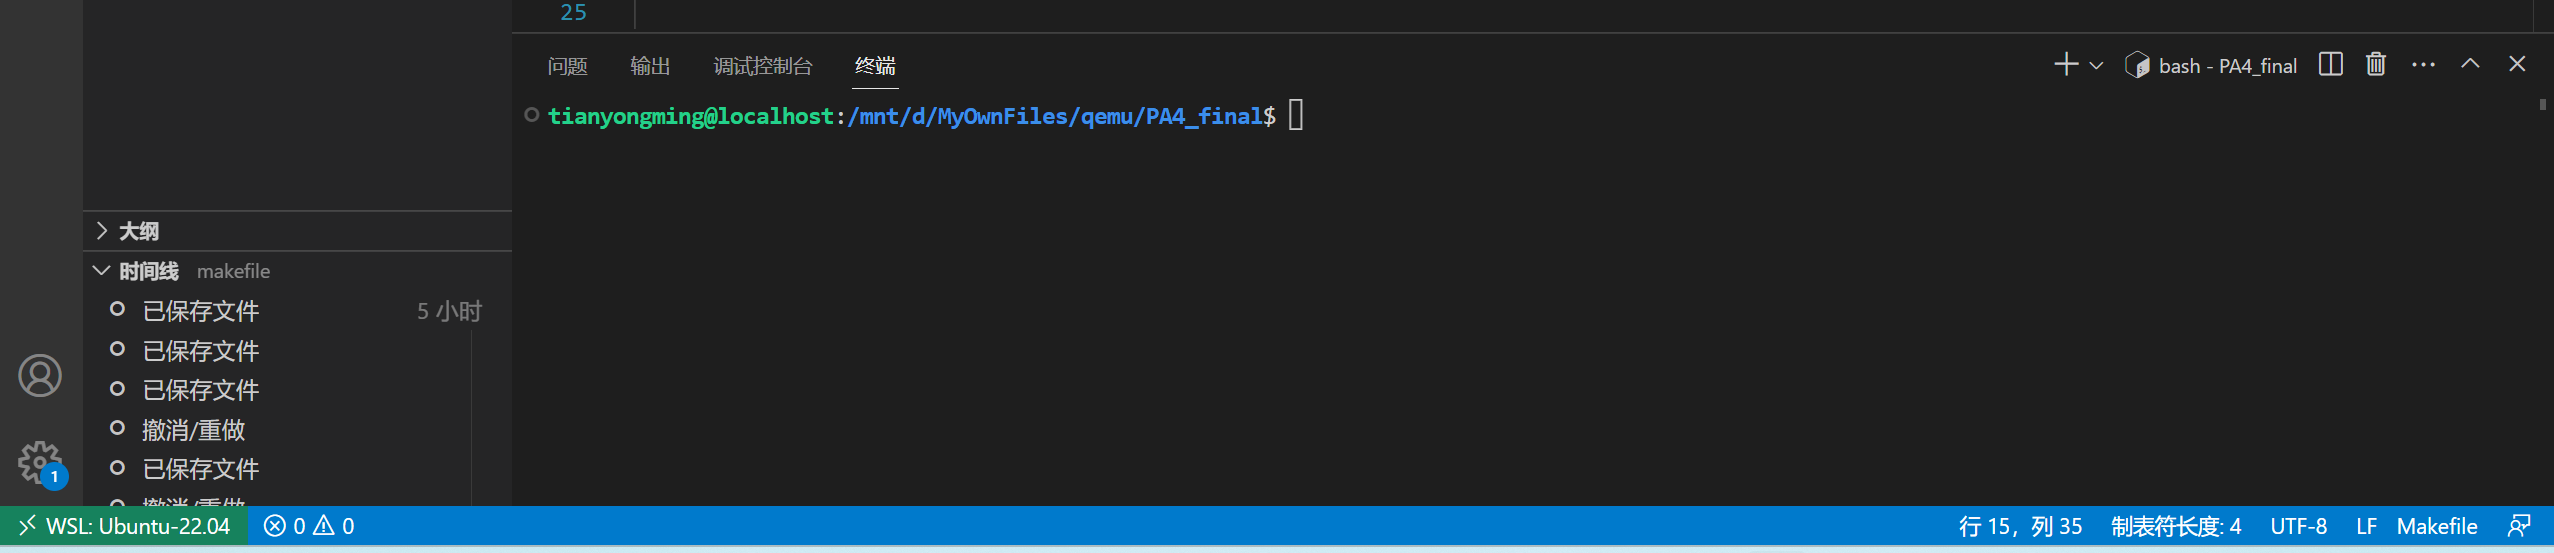
\includegraphics[width=0.7\linewidth]{C:/Users/86181/Desktop/pictures/1}
	\caption{windows-7}
	\label{fig:1}
\end{figure}

{\bf 4.再安装linux操作系统}
在qemu文件位置打开cmd,输入``qemu-system-x86\_64 -m 4096 -smp 2 myos.img -cdrom D:$\backslash$MyOwnFiles$\backslash$iso$\backslash$ubuntu-22.04.4-desktop-amd64.iso -boot d"安装linux,选择安装到之前预留的分区内。下图为安装成功的linux图片展示。

\begin{figure}[h!]
	\centering
	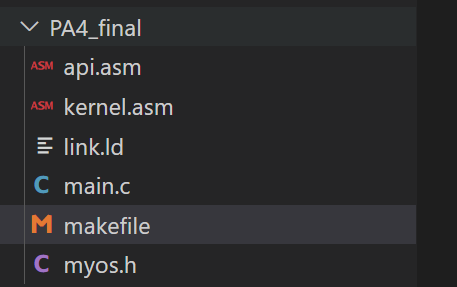
\includegraphics[width=0.7\linewidth]{C:/Users/86181/Desktop/pictures/2}
	\caption{linux}
	\label{fig:2}
\end{figure}


{\bf 5.检验安装是否成功} 再次利用命令``qemu-system-x86\_64 -m 2048 -smp 2 os.img",可以选择进入两种操作系统中的一种,分别可以成功进入。\\\\\\\\\\\\\\\\\\\

\begin{figure}[h!]
	\centering
	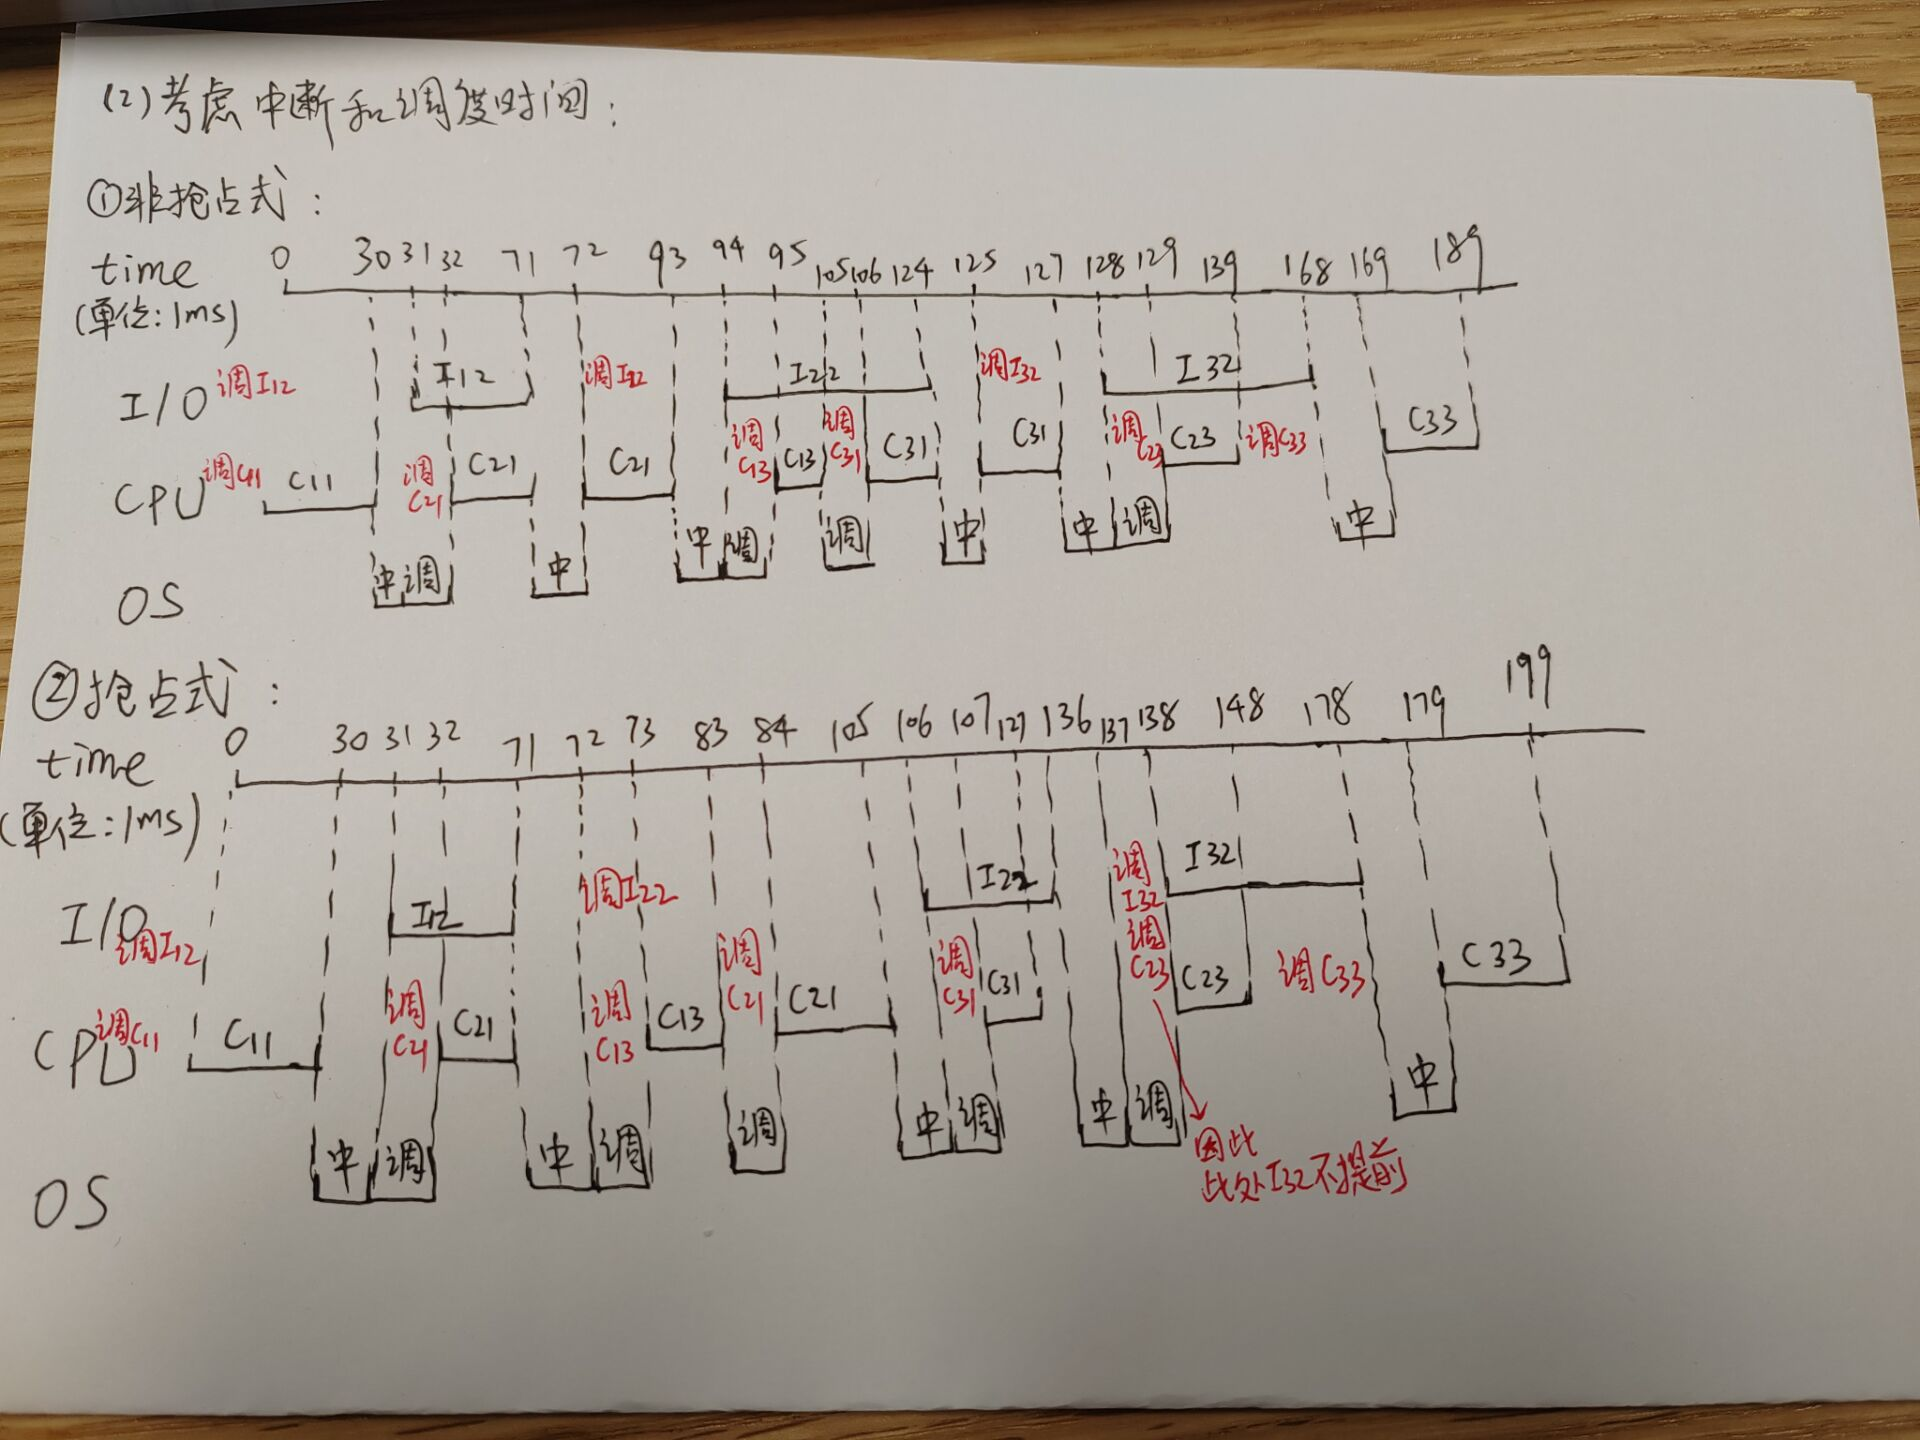
\includegraphics[width=0.7\linewidth]{C:/Users/86181/Desktop/pictures/3}
	\caption{}
	\label{fig:3}
\end{figure}

\section{读取虚拟磁盘MBR}
{\bf 1.下载工具} 通过https://xiazai.zol.com.cn/detail/47/465664.shtml下载windows的dd读取软件。

{\bf 2.进行读取} 在包含qemu的目录下创建mbr.bin,在命令行输入dd if=myos.img of=mbr.bin bs=512 count=1,打开powershell输入Format-Hex "D:/MyOwnFiles/qemu/mbr.bin",读取磁盘MBR的前512个字节。以下分别是只装了windows7和装了双系统的读的MBR:\\\\\\\\\\\\\\\\
  
\begin{figure}[h!]
	\centering
	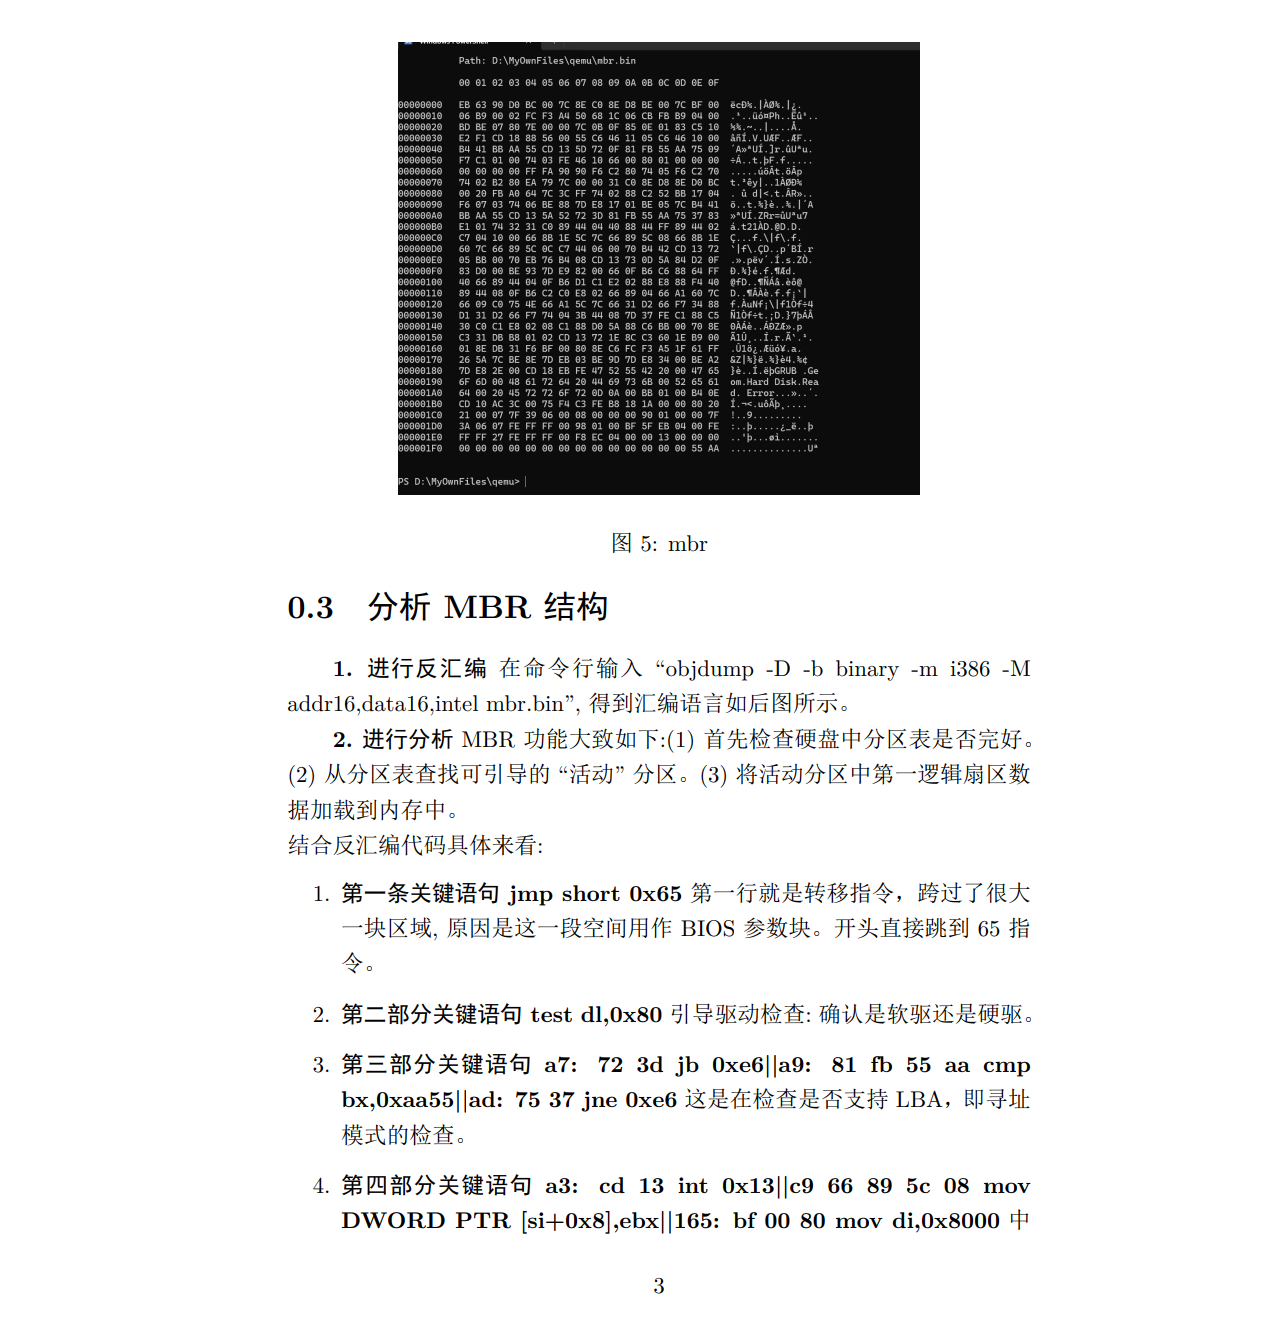
\includegraphics[width=0.7\linewidth]{C:/Users/86181/Desktop/pictures/4}
	\caption{win7-mbr}
	\label{fig:4}
\end{figure}

\begin{figure}[h!]
	\centering
	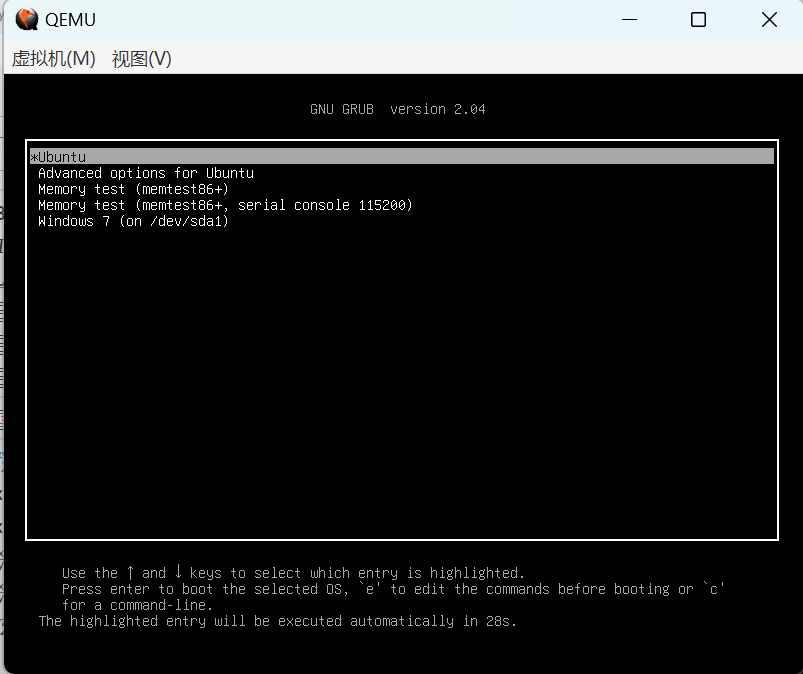
\includegraphics[width=0.7\linewidth]{C:/Users/86181/Desktop/pictures/5}
	\caption{双系统mbr}
	\label{fig:5}
\end{figure}


\section{分析MBR结构}
{\bf 1.进行反汇编} 在powershell命令行继续输入``objdump -D -b binary -m i386 -M addr16,data16,intel mbr.bin",得到mbr的汇编语言分别如后图所示(太长了,只截取了一段)。

\begin{figure}[h!]
	\centering
	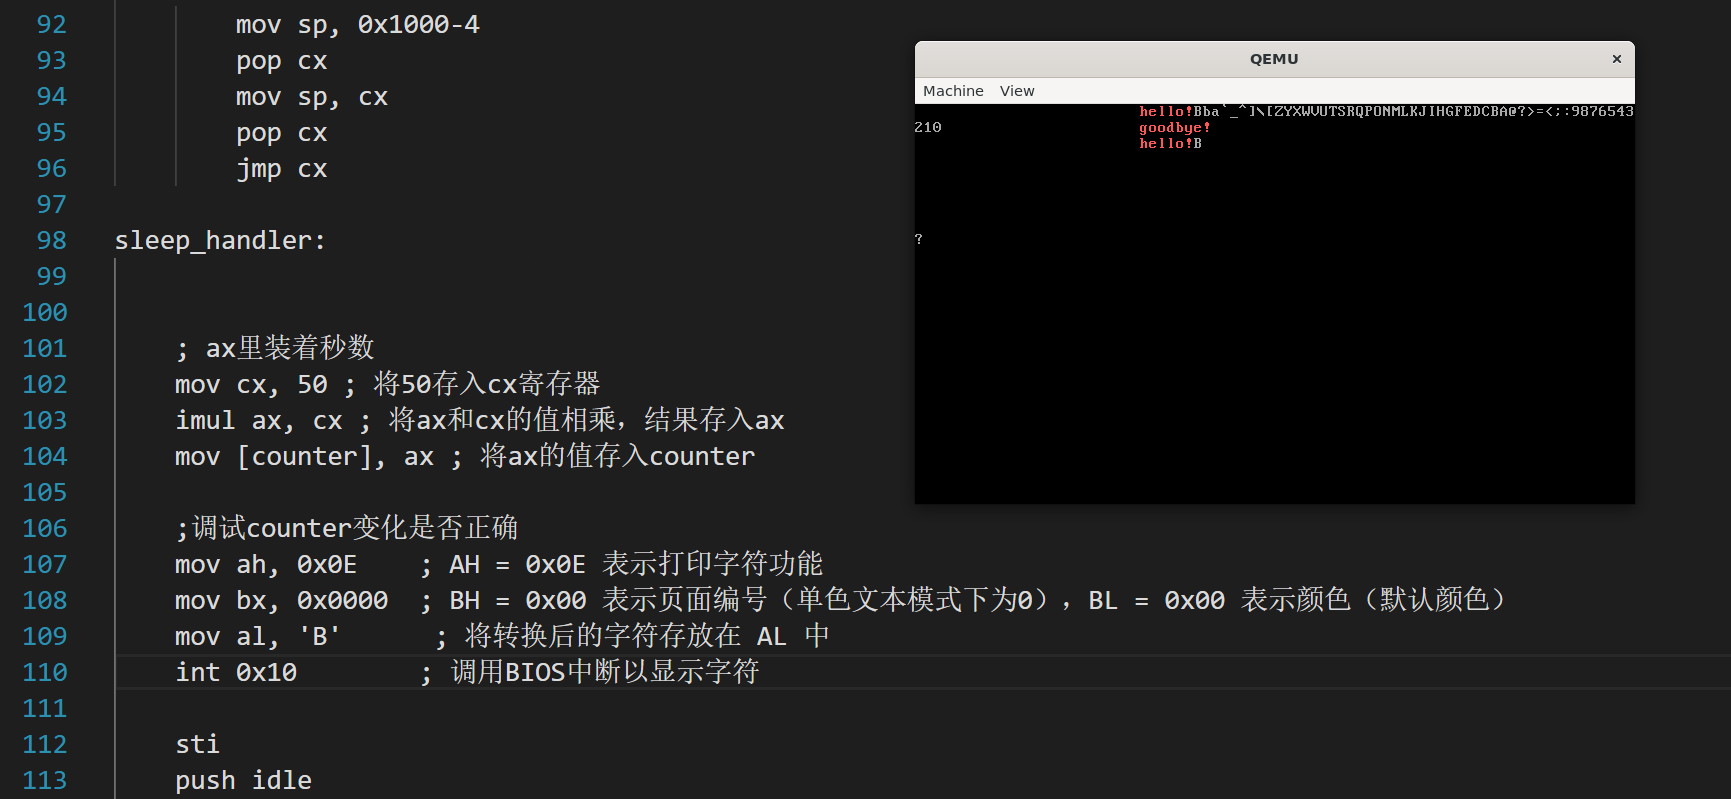
\includegraphics[width=0.7\linewidth]{C:/Users/86181/Desktop/pictures/6}
	\caption{部分反汇编结果}
	\label{fig:6}
\end{figure}

{\bf 2.进行分析}MBR功能大致如下:(1) 首先检查硬盘中分区表是否完好。(2) 从分区表查找可引导的``活动"分区。(3) 将活动分区中第一逻辑扇区数据加载到内存中。\\
结合反汇编代码具体来看:
\begin{enumerate}
	\item{\bf 第一条关键语句 jmp short 0x65} 第一行就是转移指令,跨过了很大一块区域,原因是这一段空间用作BIOS参数块。开头直接跳到65指令。
	\item{\bf 第二部分关键语句 test dl,0x80} 引导驱动检查:确认是软驱还是硬驱。
	\item{\bf 第三部分关键语句 a7: 72 3d jb 0xe6||a9: 81 fb 55 aa  cmp  bx,0xaa55||ad: 75 37 jne 0xe6} 这是在检查是否支持LBA,即寻址模式的检查。
	\item{\bf 第四部分关键语句  a3: cd 13 int 0x13||c9 66 89 5c 08   mov DWORD PTR [si+0x8],ebx||165:   bf 00 80  mov di,0x8000}中断例程启动,完成后将磁盘数据写入内存。将编号80的驱动器(c盘)的第一个扇区(512 Byte)读到内存地址。准备启动盘驱动磁盘数据包并引导内核督导内存00:8000,再执行引到内核指令。
	\item{\bf 第五部分关键语句 最后面部分(结尾是55aa)} 此部分为MBR磁盘分区表。
\end{enumerate}
	{\bf 具体来看分区部分}第1字节80是引导标志,表示为活动分区;第2、3、4字节是本分区的起始磁头号、扇区号、柱面号;第5字节是分区类型符;第6、7、8字节是分区的结束磁头号、扇区号、柱面号;第9、10、11、12字节是逻辑起始扇区号 ,本分区之前已用了的扇区数;第13、14、15、16字节是本分区的总扇区数。\\
	一个分区表能表示4个分区。以下是我的分区详细解释:\\
	{\bf 以win-7的第一块分区为例子:80 20 21 00 07 DF 13 0C 00 08 00 00 00 20 03 00} 80代表这个分区位活动分区;20,21,00表示这个分区起始扇区为16进制下的20磁头,21扇区,0柱面;07代表分区文件系统为NTFS;DF,13,0C是相应16进制下结束的磁头、扇区、柱面号;00 08 00 00 反向,$(00 00 08 00)_{16}$表示其实逻辑扇区和逻辑0扇区的差,说明前面已经有$(00 00 08 00)_{16}$个扇区;00 20 03 00表示总扇区数字。

{\bf 对比装linux前后的MBR} 经过对比,可以发现,我将linux的启动分区挂载在windows空的分区下后,原本是00(表示分区未用)的分区被linux占用。即图片中win-7情况下都是00的分区在装了linux被使用起来,有了新的数字。\\
	同时,我发现原本分区表第一个字节的80变为了00,即变成了非活动分区。\\
	再经观察,得知前两个分区的其他数字完全没有改变,这也完全符合预期,即双系统互不干扰,并没有覆盖。\\
	再对比装linux前后的汇编代码,可以发现大体相同,主要的功能都是引导作用。	
	
	{\bf 利用fdisk -l指令检验分区}在ubuntu内的终端里,输入fdisk -l,获取磁盘分区信息如下图所示:
	
\begin{figure}[h!]
	\centering
	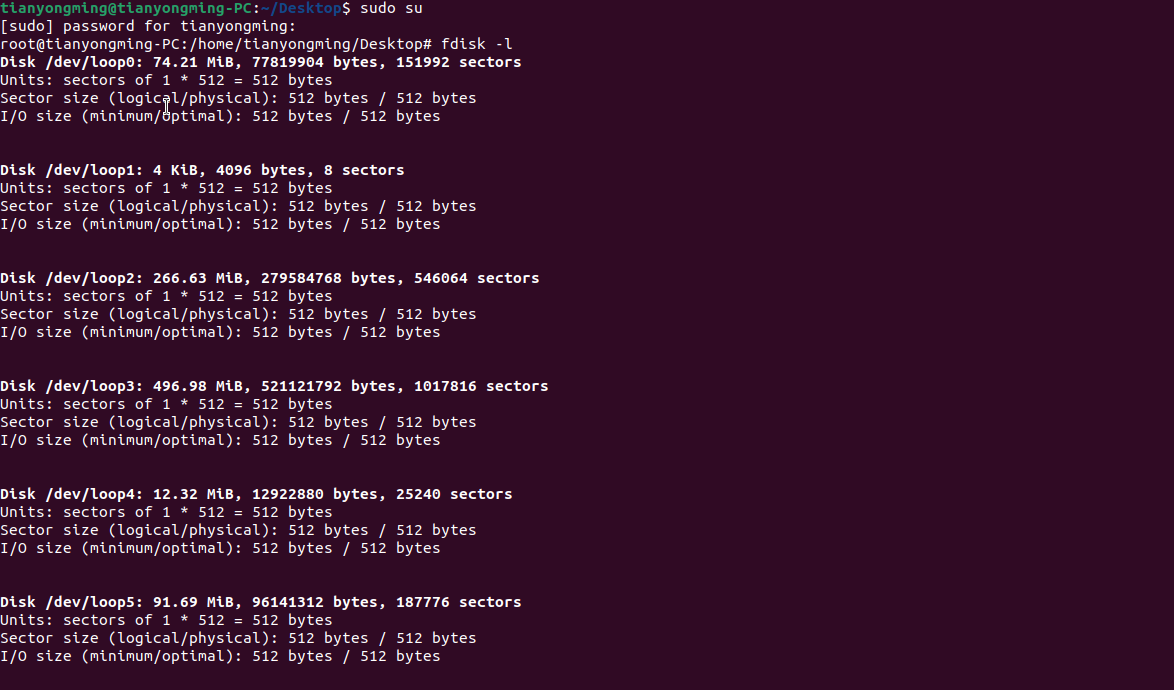
\includegraphics[width=0.7\linewidth]{C:/Users/86181/Desktop/pictures/7}
	\caption{}
	\label{fig:7}
\end{figure}

\begin{figure}[h!]
	\centering
	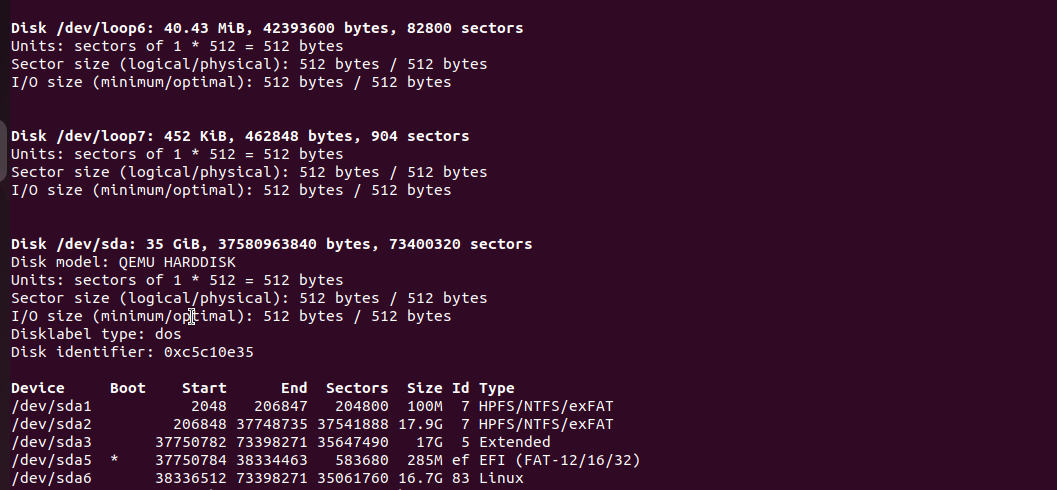
\includegraphics[width=0.7\linewidth]{C:/Users/86181/Desktop/pictures/8}
	\caption{}
	\label{fig:8}
\end{figure}

可以从图中看到我规划的分区,17.9G给window-7,16.7G给linux。更加仔细地来看,第一个sda1起始位置是2048,刚好是我的mbr读出来的$(00 00 08 00)_{16}$表示前面有多少个分区对应,这个数字在10进制下就是图片中的2048。同时,也可以通过简单的计算,将其他数字都一一对应上,这再一次验证了我读的mbr是正确的。

\end{document} 